% Options for packages loaded elsewhere
\PassOptionsToPackage{unicode}{hyperref}
\PassOptionsToPackage{hyphens}{url}
\PassOptionsToPackage{dvipsnames,svgnames,x11names}{xcolor}
%
\documentclass[
  letterpaper,
  DIV=11,
  numbers=noendperiod]{scrartcl}

\usepackage{amsmath,amssymb}
\usepackage{iftex}
\ifPDFTeX
  \usepackage[T1]{fontenc}
  \usepackage[utf8]{inputenc}
  \usepackage{textcomp} % provide euro and other symbols
\else % if luatex or xetex
  \usepackage{unicode-math}
  \defaultfontfeatures{Scale=MatchLowercase}
  \defaultfontfeatures[\rmfamily]{Ligatures=TeX,Scale=1}
\fi
\usepackage{lmodern}
\ifPDFTeX\else  
    % xetex/luatex font selection
\fi
% Use upquote if available, for straight quotes in verbatim environments
\IfFileExists{upquote.sty}{\usepackage{upquote}}{}
\IfFileExists{microtype.sty}{% use microtype if available
  \usepackage[]{microtype}
  \UseMicrotypeSet[protrusion]{basicmath} % disable protrusion for tt fonts
}{}
\makeatletter
\@ifundefined{KOMAClassName}{% if non-KOMA class
  \IfFileExists{parskip.sty}{%
    \usepackage{parskip}
  }{% else
    \setlength{\parindent}{0pt}
    \setlength{\parskip}{6pt plus 2pt minus 1pt}}
}{% if KOMA class
  \KOMAoptions{parskip=half}}
\makeatother
\usepackage{xcolor}
\setlength{\emergencystretch}{3em} % prevent overfull lines
\setcounter{secnumdepth}{-\maxdimen} % remove section numbering
% Make \paragraph and \subparagraph free-standing
\makeatletter
\ifx\paragraph\undefined\else
  \let\oldparagraph\paragraph
  \renewcommand{\paragraph}{
    \@ifstar
      \xxxParagraphStar
      \xxxParagraphNoStar
  }
  \newcommand{\xxxParagraphStar}[1]{\oldparagraph*{#1}\mbox{}}
  \newcommand{\xxxParagraphNoStar}[1]{\oldparagraph{#1}\mbox{}}
\fi
\ifx\subparagraph\undefined\else
  \let\oldsubparagraph\subparagraph
  \renewcommand{\subparagraph}{
    \@ifstar
      \xxxSubParagraphStar
      \xxxSubParagraphNoStar
  }
  \newcommand{\xxxSubParagraphStar}[1]{\oldsubparagraph*{#1}\mbox{}}
  \newcommand{\xxxSubParagraphNoStar}[1]{\oldsubparagraph{#1}\mbox{}}
\fi
\makeatother


\providecommand{\tightlist}{%
  \setlength{\itemsep}{0pt}\setlength{\parskip}{0pt}}\usepackage{longtable,booktabs,array}
\usepackage{calc} % for calculating minipage widths
% Correct order of tables after \paragraph or \subparagraph
\usepackage{etoolbox}
\makeatletter
\patchcmd\longtable{\par}{\if@noskipsec\mbox{}\fi\par}{}{}
\makeatother
% Allow footnotes in longtable head/foot
\IfFileExists{footnotehyper.sty}{\usepackage{footnotehyper}}{\usepackage{footnote}}
\makesavenoteenv{longtable}
\usepackage{graphicx}
\makeatletter
\newsavebox\pandoc@box
\newcommand*\pandocbounded[1]{% scales image to fit in text height/width
  \sbox\pandoc@box{#1}%
  \Gscale@div\@tempa{\textheight}{\dimexpr\ht\pandoc@box+\dp\pandoc@box\relax}%
  \Gscale@div\@tempb{\linewidth}{\wd\pandoc@box}%
  \ifdim\@tempb\p@<\@tempa\p@\let\@tempa\@tempb\fi% select the smaller of both
  \ifdim\@tempa\p@<\p@\scalebox{\@tempa}{\usebox\pandoc@box}%
  \else\usebox{\pandoc@box}%
  \fi%
}
% Set default figure placement to htbp
\def\fps@figure{htbp}
\makeatother
% definitions for citeproc citations
\NewDocumentCommand\citeproctext{}{}
\NewDocumentCommand\citeproc{mm}{%
  \begingroup\def\citeproctext{#2}\cite{#1}\endgroup}
\makeatletter
 % allow citations to break across lines
 \let\@cite@ofmt\@firstofone
 % avoid brackets around text for \cite:
 \def\@biblabel#1{}
 \def\@cite#1#2{{#1\if@tempswa , #2\fi}}
\makeatother
\newlength{\cslhangindent}
\setlength{\cslhangindent}{1.5em}
\newlength{\csllabelwidth}
\setlength{\csllabelwidth}{3em}
\newenvironment{CSLReferences}[2] % #1 hanging-indent, #2 entry-spacing
 {\begin{list}{}{%
  \setlength{\itemindent}{0pt}
  \setlength{\leftmargin}{0pt}
  \setlength{\parsep}{0pt}
  % turn on hanging indent if param 1 is 1
  \ifodd #1
   \setlength{\leftmargin}{\cslhangindent}
   \setlength{\itemindent}{-1\cslhangindent}
  \fi
  % set entry spacing
  \setlength{\itemsep}{#2\baselineskip}}}
 {\end{list}}
\usepackage{calc}
\newcommand{\CSLBlock}[1]{\hfill\break\parbox[t]{\linewidth}{\strut\ignorespaces#1\strut}}
\newcommand{\CSLLeftMargin}[1]{\parbox[t]{\csllabelwidth}{\strut#1\strut}}
\newcommand{\CSLRightInline}[1]{\parbox[t]{\linewidth - \csllabelwidth}{\strut#1\strut}}
\newcommand{\CSLIndent}[1]{\hspace{\cslhangindent}#1}

\KOMAoption{captions}{tableheading}
\makeatletter
\@ifpackageloaded{caption}{}{\usepackage{caption}}
\AtBeginDocument{%
\ifdefined\contentsname
  \renewcommand*\contentsname{Table of contents}
\else
  \newcommand\contentsname{Table of contents}
\fi
\ifdefined\listfigurename
  \renewcommand*\listfigurename{List of Figures}
\else
  \newcommand\listfigurename{List of Figures}
\fi
\ifdefined\listtablename
  \renewcommand*\listtablename{List of Tables}
\else
  \newcommand\listtablename{List of Tables}
\fi
\ifdefined\figurename
  \renewcommand*\figurename{Figure}
\else
  \newcommand\figurename{Figure}
\fi
\ifdefined\tablename
  \renewcommand*\tablename{Table}
\else
  \newcommand\tablename{Table}
\fi
}
\@ifpackageloaded{float}{}{\usepackage{float}}
\floatstyle{ruled}
\@ifundefined{c@chapter}{\newfloat{codelisting}{h}{lop}}{\newfloat{codelisting}{h}{lop}[chapter]}
\floatname{codelisting}{Listing}
\newcommand*\listoflistings{\listof{codelisting}{List of Listings}}
\makeatother
\makeatletter
\makeatother
\makeatletter
\@ifpackageloaded{caption}{}{\usepackage{caption}}
\@ifpackageloaded{subcaption}{}{\usepackage{subcaption}}
\makeatother

\usepackage{bookmark}

\IfFileExists{xurl.sty}{\usepackage{xurl}}{} % add URL line breaks if available
\urlstyle{same} % disable monospaced font for URLs
\hypersetup{
  pdftitle={DSCI 310: Historical Horse Population in Canada},
  pdfauthor={Tiffany Timbers \& Jordan Bourak},
  colorlinks=true,
  linkcolor={blue},
  filecolor={Maroon},
  citecolor={Blue},
  urlcolor={Blue},
  pdfcreator={LaTeX via pandoc}}


\title{DSCI 310: Historical Horse Population in Canada}
\author{Tiffany Timbers \& Jordan Bourak}
\date{}

\begin{document}
\maketitle


\subsection{Aim}\label{aim}

This project explores the historical population of horses in Canada
between 1906 and 1972 for each province.

\subsection{Data}\label{data}

Horse population data were sourced from the
\href{http://open.canada.ca/en/open-data}{Government of Canada's Open
Data website} (Government of Canada (2017a); Government of Canada
(2017b)).

\subsection{Methods}\label{methods}

The Python programming language (Van Rossum and Drake (2009)) and the
following Python packages were used to perform the analysis: pandas
(McKinney (2010)), altair (VanderPlas (2018)), click (Team (2020)), as
well as Quarto (Allaire et al. (2022)). \emph{Note: this report is
adapted from (Timbers (2020)).}

\subsection{Results}\label{results}

\begin{figure}

\centering{

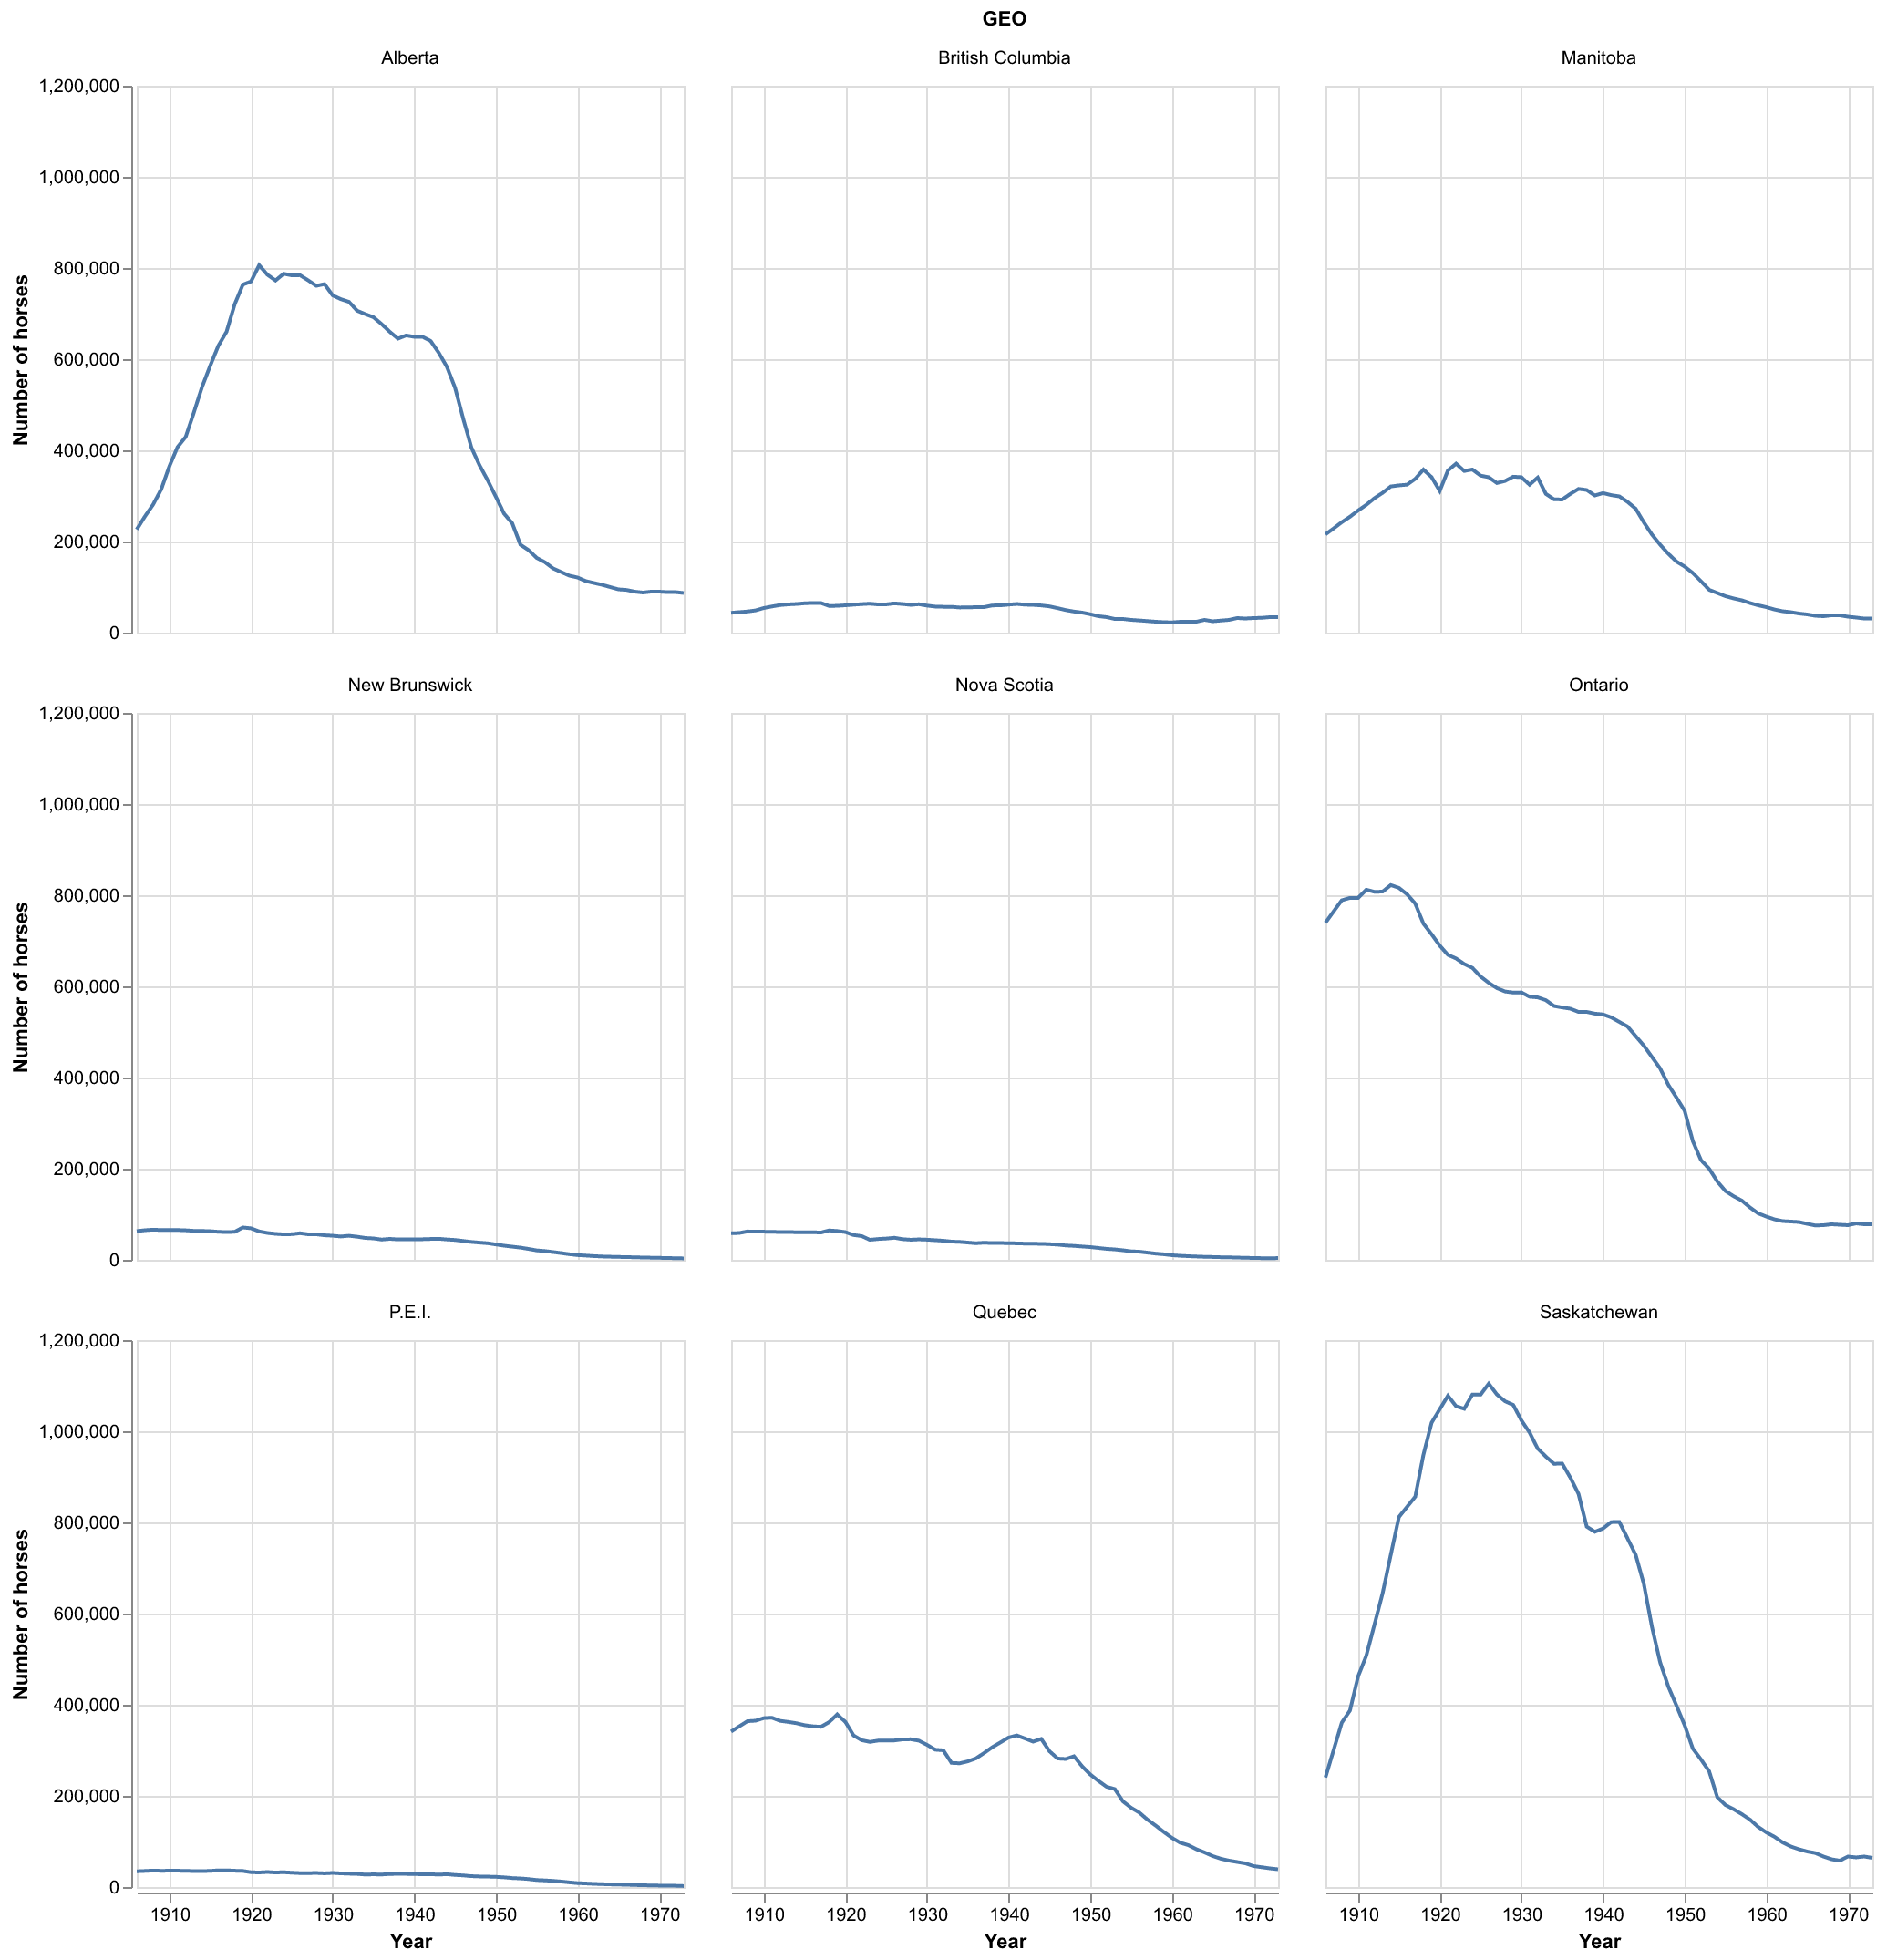
\includegraphics[width=0.7\linewidth,height=\textheight,keepaspectratio]{../results/horse_pops_plot.png}

}

\caption{\label{fig-horse-pop}Horse populations for all provinces in
Canada from 1906 - 1972}

\end{figure}%

We can see from Figure~\ref{fig-horse-pop} that Ontario, Saskatchewan
and Alberta have had the highest horse populations in Canada. All
provinces have had a decline in horse populations since 1940. This is
likely due to the rebound of the Canadian automotive industry after the
Great Depression and the Second World War. An interesting follow-up
visualisation would be car sales per year for each Province over the
time period visualised above to further support this hypothesis.

Suppose we were interested in looking in more closely at the province
with the highest spread (in terms of standard deviation) of horse
populations. We present the standard deviations in (\textbf{table1?}).

\begin{longtable}[]{@{}lr@{}}
\toprule\noalign{}
Province & Std \\
\midrule\noalign{}
\endhead
\bottomrule\noalign{}
\endlastfoot
Saskatchewan & 377266 \\
Ontario & 266435 \\
Alberta & 266063 \\
Manitoba & 122404 \\
Quebec & 111411 \\
New Brunswick & 22019.5 \\
Nova Scotia & 19879.3 \\
British Columbia & 14945.7 \\
P.E.I. & 11355.7 \\
\end{longtable}

\begin{figure}

{\centering \includegraphics[width=0.65\linewidth,height=\textheight,keepaspectratio]{../results/horses_sd.csv}

}

\caption{Standard deviation of historical (1906-1972) horse populations
for each Canadian province}

\end{figure}%

Note that we define standard deviation (of a sample) as

\[s = \sqrt{\frac{\sum_{i=1}^N (x_i - \overline{x})^2}{N-1} }\]

Additionally, note that in (\textbf{table1?}) we consider the sample
standard deviation of the number of horses during the same time span as
Figure~\ref{fig-horse-pop}.

\begin{figure}

\centering{

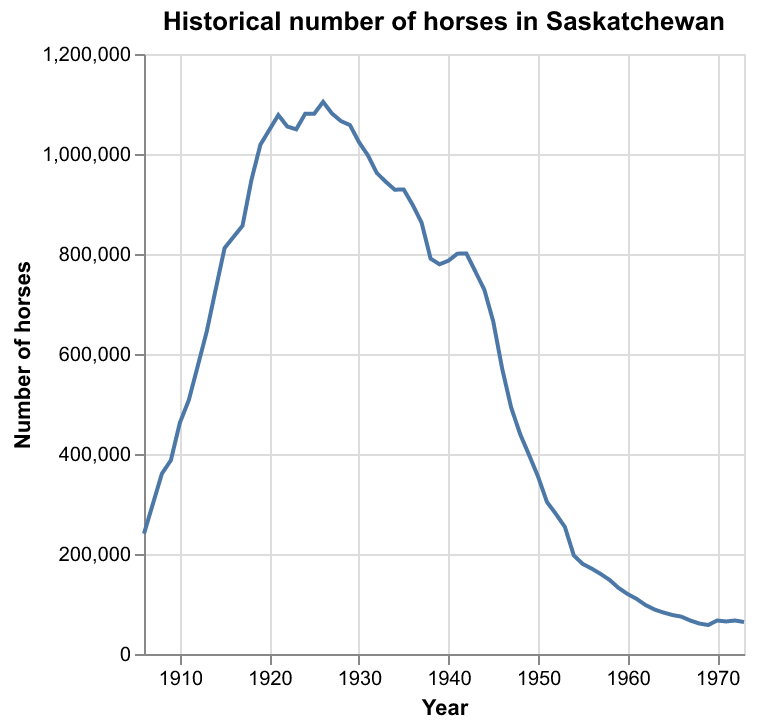
\includegraphics[width=0.65\linewidth,height=\textheight,keepaspectratio]{../results/horse_pops_plot_largest_sd.png}

}

\caption{\label{fig-largest-sd}Horse populations for the province with
the largest standard deviation}

\end{figure}%

In Figure~\ref{fig-largest-sd} we zoom in and look at the province of
\texttt{\{largest\_sd\_province\}}, which had the largest spread of
values in terms of standard deviation.

\subsection*{References}\label{references}
\addcontentsline{toc}{subsection}{References}

\phantomsection\label{refs}
\begin{CSLReferences}{1}{0}
\bibitem[\citeproctext]{ref-Allaire_Quarto_2022}
Allaire, J. J., Charles Teague, Carlos Scheidegger, Yihui Xie, and
Christophe Dervieux. 2022. {``{Quarto}.''}
\url{https://doi.org/10.5281/zenodo.5960048}.

\bibitem[\citeproctext]{ref-horses1}
Government of Canada. 2017a. {``Horses, Number on Farms at June 1 and at
December 1.''} Open Government - Open Data.
\url{https://open.canada.ca/data/en/dataset/a3ecf553-8ec4-4551-a0fe-8df1472c6cf7}.

\bibitem[\citeproctext]{ref-horses2}
---------. 2017b. {``Horses, Number on Farms at June 1, Farm Value Per
Head and Total Farm Value.''} Open Government - Open Data.
\url{https://open.canada.ca/data/en/dataset/e175ef9c-98f0-49b3-8131-ca0e3895a0cb}.

\bibitem[\citeproctext]{ref-pandas}
McKinney, Wes. 2010. {``Data Structures for Statistical Computing in
Python.''} In \emph{Proceedings of the 9th Python in Science
Conference}, edited by Stéfan van der Walt and Jarrod Millman, =51--56.

\bibitem[\citeproctext]{ref-click}
Team, Pallets. 2020. \emph{Click}.
\url{https://click.palletsprojects.com/}.

\bibitem[\citeproctext]{ref-ttimbers-horses}
Timbers, Tiffany. 2020. \emph{Historical Horse Population in Canada}.
\url{https://github.com/ttimbers/equine_numbers_value_canada_parameters}.

\bibitem[\citeproctext]{ref-Python}
Van Rossum, Guido, and Fred L. Drake. 2009. \emph{Python 3 Reference
Manual}. Scotts Valley, CA: CreateSpace.

\bibitem[\citeproctext]{ref-altair}
VanderPlas, Jake. 2018. {``Altair: Interactive Statistical
Visualizations for Python.''} \emph{Journal of Open Source Software} 3
(7825, 32): 1057. \url{https://doi.org/10.21105/joss.01057}.

\end{CSLReferences}




\end{document}
